\documentclass{article}
\usepackage[utf8]{inputenc}
\usepackage[sc]{mathpazo}
\usepackage{graphicx}
\usepackage{url}
\usepackage{hyperref}
\usepackage{subcaption}
\usepackage{svg}
\usepackage[style=numeric]{biblatex}

\graphicspath{ {./images/} }

\title{Preventing Secondary Structure Formation in the ADS Codex}
\author{Alina Li}
\date{Aug 5, 2022}

\begin{document} 
\maketitle

\begin{abstract}
In the field of bioinformatics, the formation of secondary structures increases the likelihood of DNA sequencing errors. In this paper, we explore how to prevent secondary structure formation in the context of DNA data storage. We contribute to the ADS codex, an open-source DNA codec, by integrating nucleic acid structure analysis to reduce the number of sequences with prominent secondary structures. We use random seeds and data randomization to produce variation in secondary structure prevalence, and found that the effect was minimal. We discuss next steps for secondary structure prevention in the codec.
\end{abstract}

\section{Introduction}
DNA data storage is an exciting field of research because it could reduce the need for traditional physical media in the coming decades. In the future, our digital data could be stored in DNA rather than hard drives, which has a number of advantages. First, DNA has high data density, in part due to the small and condensed nature of the molecule [1]. In 2017, for instance, researchers at Columbia University were able to encode 215 petabytes of data in a gram of DNA [5]. That data density could reach even higher values as technology advances. In addition to high data density, DNA data storage is also very scalable. Hardware changes over time whereas DNA remains the same -- a biological molecule that relies on common chemical processes for synthesis and sequencing.  

However, various obstacles prevent its adoption, including high costs and sequencing and synthesis errors [1]. Costs are not a major concern -- the cost of sequencing DNA (the process of determining the order of nucleotides), for instance, has been steadily decreasing over the past two decades (Figure 1) [4]. High error rates do exist and will continue to exist, necessitating the development of methods to avoid and fix errors specific to DNA. Insertion, deletion, and substitution errors are some examples [1]. DNA codecs must be able to work around or fix these errors, or else fail to fully recover data. Currently, most codecs, including the ADS codex, avoids errors resulting from problematic sequences, such as those with a higher content of C and G nucleotides and homopolymers (sequences of a repeating base). These problematic sequences increase the likelihood of sequencing or synthesis error. 

Most codecs, however, have not yet developed methods to avoid encoding sequences with prominent secondary structures, which increase error rates [1].

\begin{figure}
\centering
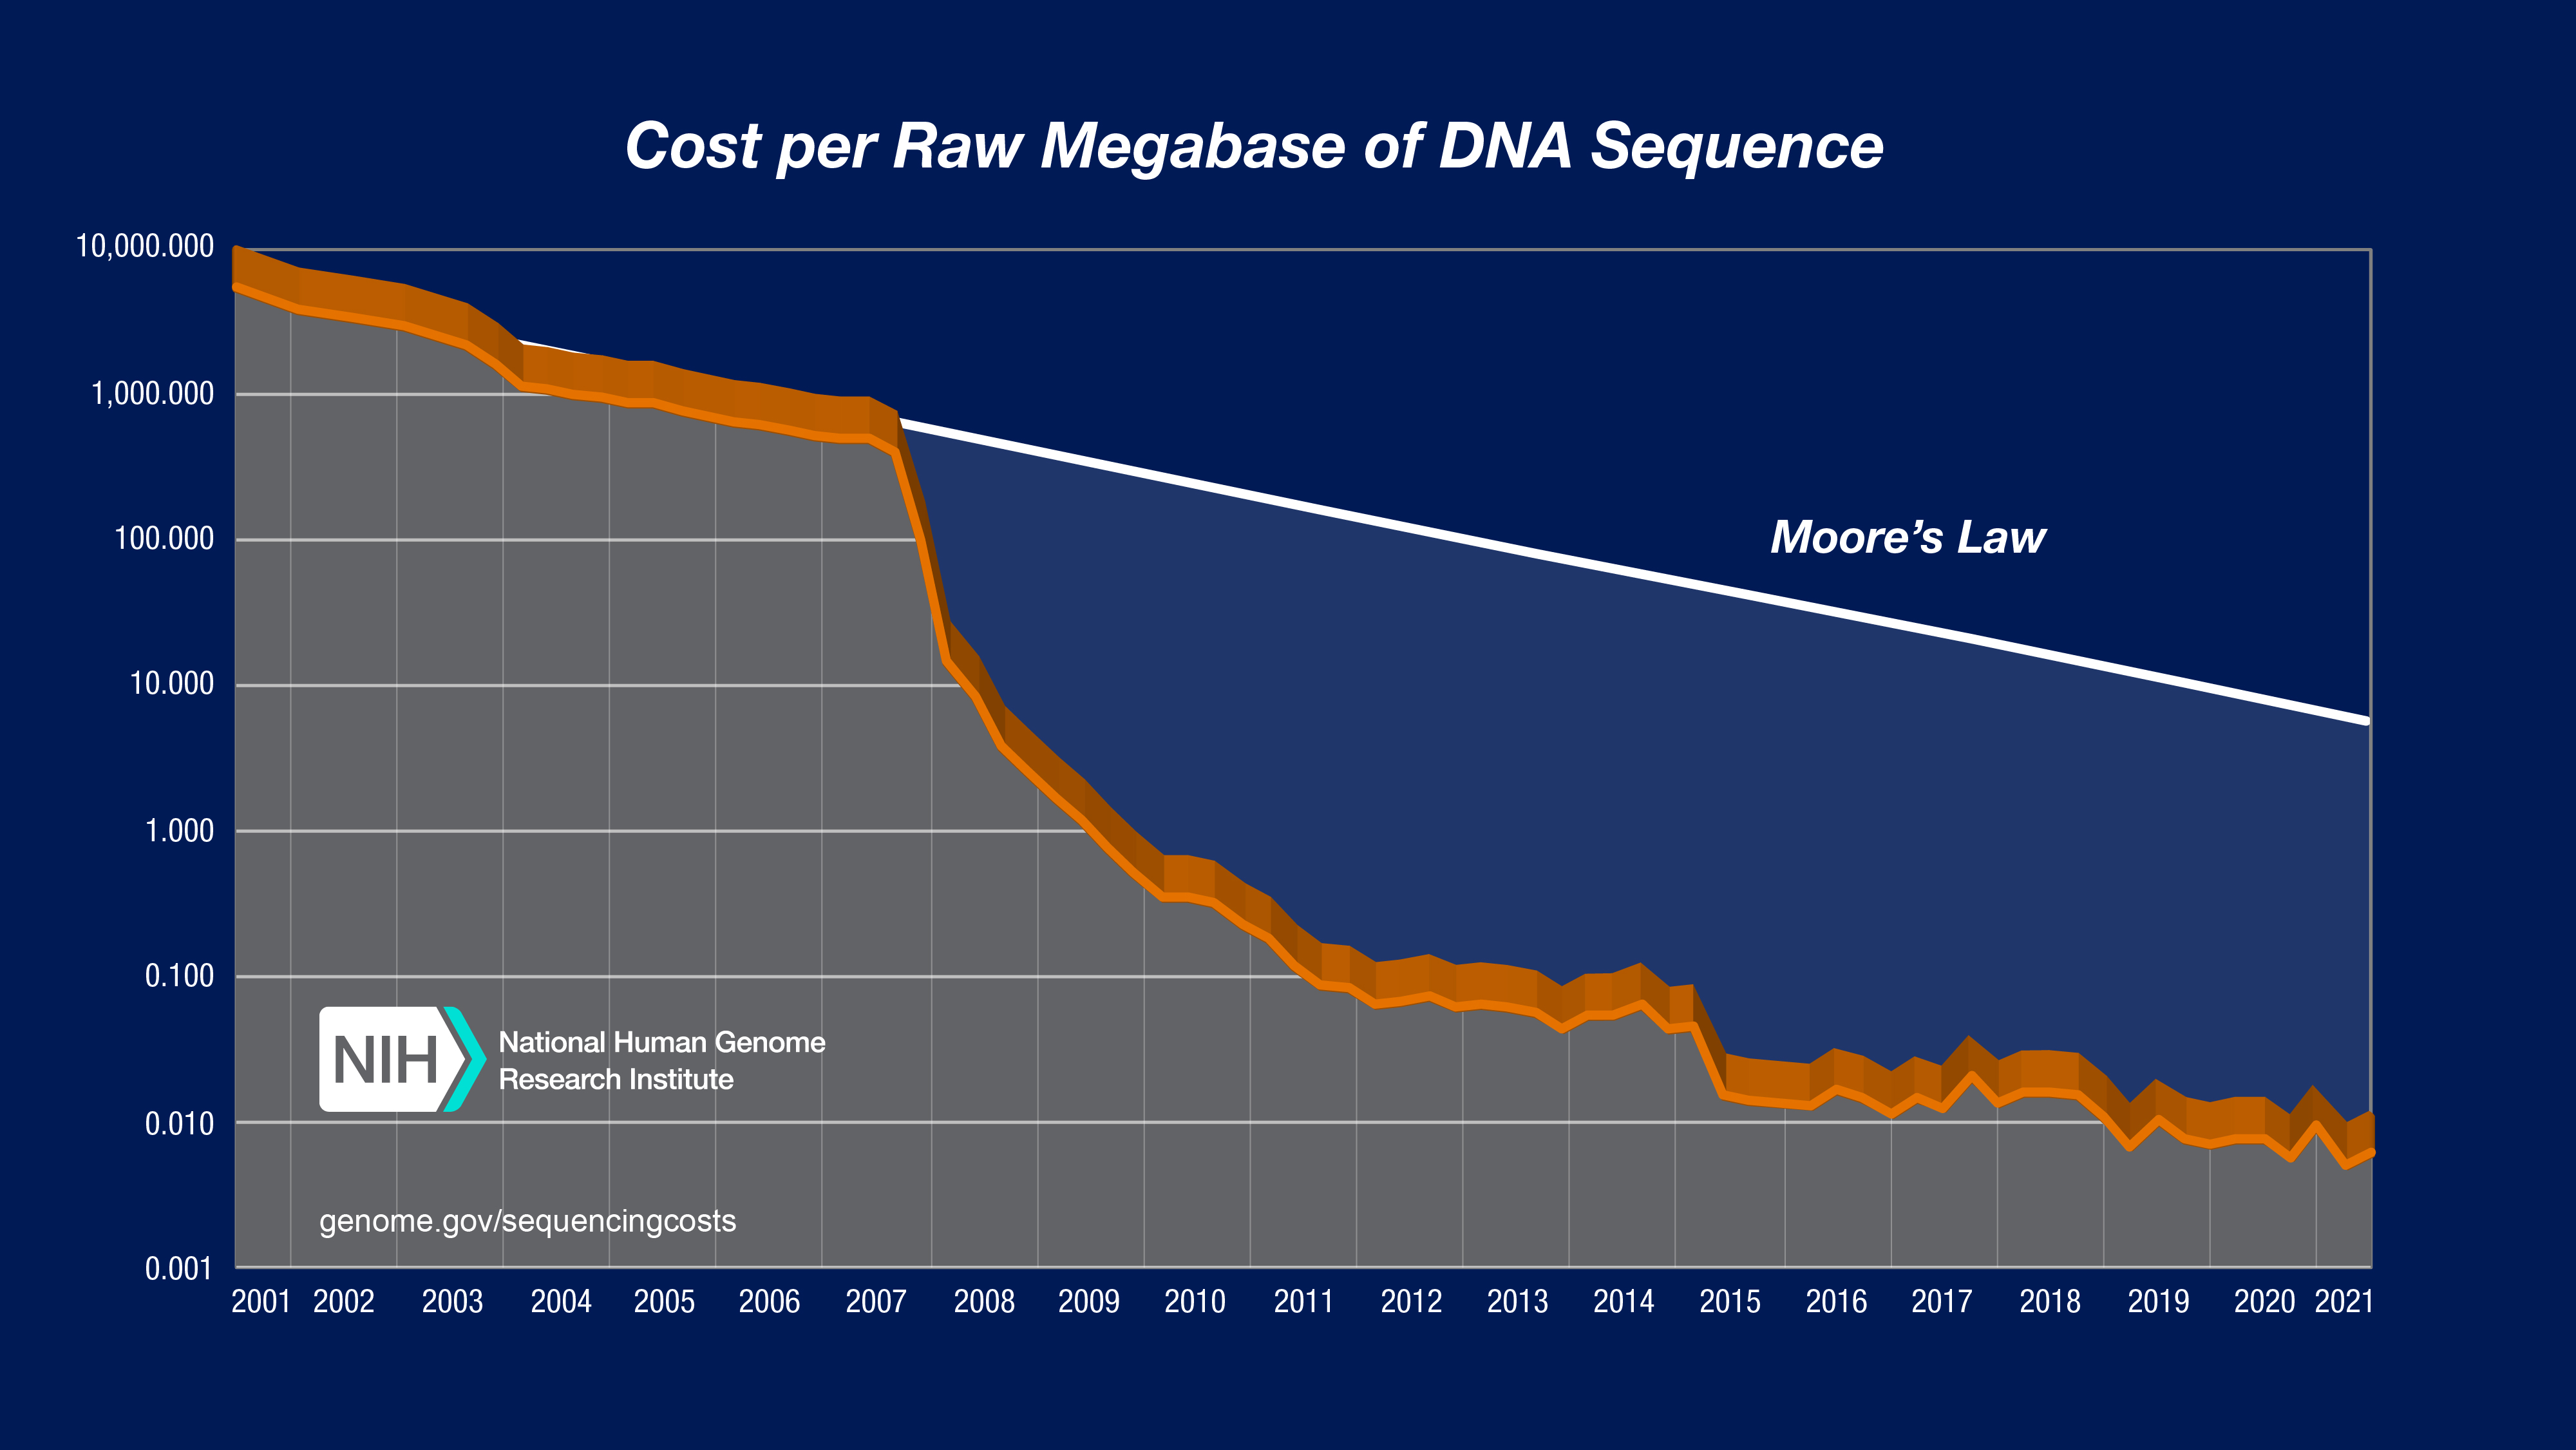
\includegraphics[width=\textwidth]{2021_sequencing_cost_per_Mb.jpg}
\caption{Sequencing cost per Megabase of DNA from \url{https://www.genome.gov/about-genomics/fact-sheets/DNA-Sequencing-Costs-Data}}
\end{figure}

Our project attempts to fix the lack of secondary structure prevention in DNA codecs. We chose to contribute to the ADS codex, a recently developed open-source codec. The aim is to reduce secondary structure formation, and thus, reduce error rates and improve data recovery. In the following sections, we give background on secondary structures and the software package NUPACK, which contains functionality for performing secondary structure analysis [3]. We also describe how DNA analysis could be integrated into the ADS codex in the future. Finally, we describe our results and outline areas where further research is needed.

\section{DNA Analysis}
DNA, a two-stranded molecule, has a helical secondary structure, where the two strands' base pairs complement each other. For the purposes of this paper, when we refer to DNA strands, we are discussing single strands of DNA, or oligos. These oligos are sequences of four different nucleotides -- adenine, cytosine, guanine, and thymine. Due to nucleotide base pair interactions, oligos can form secondary structures. Secondary structures occur when complementary sections of the strand connect to each other, forming structures such as hairpin loops, stacking pairs, and others (Figure 2). 

\begin{figure}[!h]
\centering
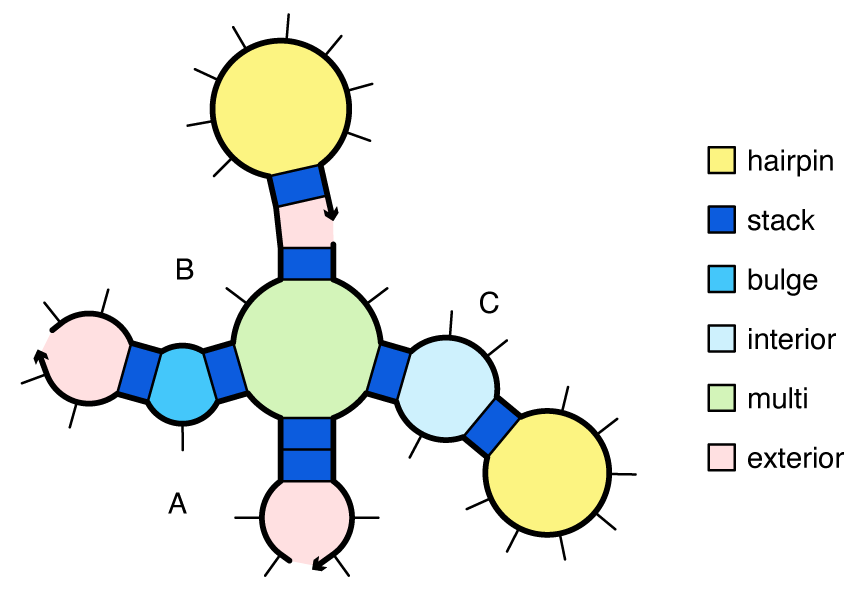
\includegraphics[scale=1]{secondary_structures_overview.png}
\caption{Examples of secondary structures from \url{https://docs.nupack.org/definitions}}   
\end{figure} 


Generally speaking, a given strand has the ability to form multiple different secondary structures. Some structures are more prominent than others (ie. due to number and strength of bonds), meaning that they are more likely to interfere with sequencing. Quantitatively, we can compare secondary structures by calculating their free energy, a measure based on base pair interactions. Free energy measures the ability for a system to change, and in this case, it measures the change in energy from the unfolded state with no interactions to the secondary structure state. Smaller values mean that the structure is more prominent [2]. In Figure 3, two secondary structures from two DNA sequences are shown. The structures have different free energies. The secondary structure in Figure 3a has a smaller free energy, and the physical differences are obvious. The equilibrium probabilities of the bonded nucleotides are close to one, indicating a higher chance of remaining bonded, and, a higher proportion of nucleotides are in the bonded state.

The formation of prominent secondary structures reduces the ability for the strand to be successfully sequenced. The two most popular sequencing technologies, sequencing by synthesis and sequencing by nanopores, for instance, fail to sequence when it encounters a hairpin loop.

Therefore, comparison of secondary structure and their free energy is essential to improve data recovery for the ADS codex. 

\begin{figure}[!h]
\centering
\begin{subfigure}{.5\textwidth}
  \centering
  \includesvg[scale=.5]{mfe_low.svg}
  \caption{Small free energy}
  \label{fig:sub1}
\end{subfigure}%
\begin{subfigure}{.5\textwidth}
  \centering
  \includesvg[scale=.5]{mfe_high.svg}
  \caption{Larger free energy}
  \label{fig:sub2}
\end{subfigure}
\caption{Secondary structures with different free energies. Images generated by NUPACK}
\label{fig:test}
\end{figure}

Since a given strand can form many different secondary structures, we must have a method for determining which secondary structure to use a point of comparison against the secondary structure(s) of other strands. Conveniently, NUPACK, a software package for analyzing nucleic acid sequences, can calculate the MFE (minimum free energy) of a given strand. The MFE is the free energy of the secondary structure with the smallest (ie. most negative) free energy. Therefore, the MFE can serve as a useful metric for determining which strand has the most prominent secondary structure.

Then, given a strand's MFE, we need a heuristic to determine whether the oligo will be unideal for sequencing and synthesis. One heuristic is physics-based. A given strand can either be in the folded or extended state, where the folded state is the secondary structure. Thermodynamic analysis calculations say that the free energy threshold between the folded and extended state is equal to $-ln(f_0) * k_B * T$, where $f_0$ is the fraction of folded molecules, $k_B$ is Boltzmann’s constant, and $T$ is the temperature of the strands [2]. The details of the calculations are irrelevant for our purposes, as all we need is the threshold of free energy.

An alternative heuristic relies on data from previous research experiments. One might consider the oligos that failed to be sequenced during real experiments and calculate their free energy, using that data to determine an appropriate threshold.

\section{Integration}

With the ADS codex, our goal is to encode the data in such a way that reduces the effect of prominent secondary structures in the encoded data. If the encoded DNA strands have prominent secondary structures that result in increased sequencing and synthesis error rates, the data may be difficult to recover from the DNA strands.

The ADS codex is designed as follows: A lookup table corresponds a bit sequence composed of 1's and 0's to a nucleotide sequence in the 4-letter DNA alphabet. At its most basic level, data is converted into DNA strands using this lookup table. Before encoding, however, the data is randomized using the XOR process and a psuedorandom number generator (PRNG) to reduce the occurrence of long homopolymers. PRNGs is very appropriate for this use case -- by selecting a certain initial "seed", the PRNG produces a "random" sequence that can be replicated by using the same seed again. Therefore, though the data is randomized with the values generated by the PRNG, the data can be unrandomized during the decoding process by seeding the PRNG with the initial encoding seed. Values from the PRNG are XORed with each successive byte of data. XOR is a bit-wise operation -- given two bits, the resulting bit is 1 if the two bits are different, and 0 if the two bits are the same. Like PRNG, XOR is useful for the decoding process as A XOR B = C also means C XOR A = B, where A is the PRNG-generated value, B is the data, and C is the randomized data. Using these two methods, the initial unrandomized data is recoverable from the randomized data. 

To apply this to secondary structure analysis, this method of data randomization means that choosing different random seeds will affect the bit sequence, in turn affecting the encoded DNA sequence, and in turn affecting the MFE of the sequence. Theoretically, after running the encoder with various random seeds, we may be able to choose the "best" random seed that produces an ideal set of encoded DNA strands with minimized secondary structure prevalence. 

Methods for random seed selection assume the following process:
\begin{itemize}
    \item Run the ADS encoder with a specified random seed and receive the output -- a list of encoded DNA strands.
    \item Run NUPACK's MFE calculation on each DNA strand.
    \item After running the encoder on various random seeds, determine the best random seed using some method of comparison.
\end{itemize}

Three methods to choose the best random seed are described below:

\begin{enumerate}
    \item Take the average MFE. Choose the random seed with the least negative average MFE.
    \item Determine the percentage of "bad" oligos based on the heuristic described in the previous section. Choose the random seed with the lowest percentage of bad oligos.
    \item Determine the bad oligos based on the heuristic. Determine the disposability of these oligos that will likely get lost during the sequencing/synthesis processes. Choose the random seed where losing those bad oligos has the least impact on data recovery. (Since the ADS codex has an erasure codes for recovering data, this method takes advantage of that feature.) 
\end{enumerate}

\section{Results}

For our tests, we generated a random 32k byte file and ran the ADS encoder on it, specifying a different random seed each time. The encoder generated a list of 2740 encoded DNA strands, which we then ran NUPACK's MFE calculation on. The results of the tests are shown in Figures 4 and 5. There is a miniscule variation in average MFE, minimum MFE, and maximum MFE even across the different random seeds (Figure 4). For average MFE, the highest and lowest average differed by a mere 115 thousandths kcal/mol. Minimum MFE differed by 3.690, and maximum MFE differed by 544 thousandths. Furthermore, across all four random seeds, the distribution of MFEs fell into similar bell-curves (Figure 5).

\begin{figure}[!h]
\centering
\begin{tabular}{|c|c|c|c|}
\hline
 random seed & average MFE & min MFE & max MFE \\ 
 \hline
 approx. 32000	& -14.094 & -29.440 & -5.266 \\
 1 & -14.192 & -28.200 & -5.810 \\
 10 & -14.209 & -28.010 & -5.490 \\
 50 & -14.188 & -31.700 & -5.360 \\
 \hline
\end{tabular}
\caption{Four random seed tests run on a 32k byte file. The random seeds produced very similar MFE distributions.}
\end{figure}

\begin{figure}[!h]
\centering
\begin{subfigure}{.5\textwidth}
  \centering
  \includesvg[scale=.4]{mfe_histogram_default.svg}
  \caption{Default random seed}
  \label{fig:histogram_a}
\end{subfigure}%
\begin{subfigure}{.5\textwidth}
  \centering
  \includesvg[scale=.4]{mfe_histogram_1.svg}
  \caption{Random seed 1}
  \label{fig:histogram_b}
\end{subfigure}

\begin{subfigure}{.5\textwidth}
  \centering
  \includesvg[scale=.4]{mfe_histogram_10.svg}
  \caption{Random seed 10}
  \label{fig:histogram_c}
\end{subfigure}%
\begin{subfigure}{.5\textwidth}
  \centering
  \includesvg[scale=.4]{mfe_histogram_50.svg}
  \caption{Random seed 50}
  \label{fig:histogram_d}
\end{subfigure}
\caption{Histograms of MFE values after encoding 32k byte file with specified PRNG seeds of the default value (approximately 32000), 1, 10, and 50.}
\label{fig:test}
\end{figure}


These results indicate that selecting the random seed by comparing average, minimum, or maximum MFE may not be particularly effective. Future work should focus on refining the method of random seed selection to minimize secondary structure interference.


\section{Conclusion}

Future research might explore more advanced methods of choosing a random seed, such as considering oligo disposability. It might refine a heuristic to determine the bad oligos. These secondary structure analyses would have to be fully integrated with the codex such that the encoder can run multiple tests with different random seeds and seamlessly output the most ideal encoded DNA strands. 

After integration, tests with real DNA will also help determine whether secondary structure analysis is able to affect the error rates of the sequencing and synthesis processes, and more broadly, the DNA data storage process.


\begin{thebibliography}{5}
\bibitem{ionkov}
Ionkov, L. A. (n.d.). DNA Storage with ADS Codex: the Adaptive Codec for Organic Molecular Archives. \textit{Unpublished.} 

\bibitem{dirks}
Dirks, R. M., Bois, J. S., Schaeffer, J. M., Winfree, E., \& Pierce, N. A. (2007). Thermodynamic analysis of interacting nucleic acid strands. \textit{SIAM Review, 49}(1), 65–88. https://doi.org/10.1137/060651100 

\bibitem{nupack}
The NUPACK Team. (2021). NUPACK 4.0 User Guide. Retrieved from https://docs.nupack.org 

\bibitem{genomegov}
Wetterstrand, K. A. (n.d.). DNA Sequencing Costs: Data from the NHGRI Genome Sequencing Program (GSP). Retrieved from www.genome.gov/sequencingcostsdata

\bibitem{dnafountain}
Erlich, Y., \& Zielinski, D. (2017). DNA fountain enables a robust and efficient storage architecture. \textit{Science, 355}(6328), 950–954. https://doi.org/10.1126/science.aaj2038 

\end{thebibliography}


\end{document}